\documentclass[10pt]{article}
\usepackage[polish]{babel}
\usepackage[utf8]{inputenc}
\usepackage[T1]{fontenc}
\usepackage{amsmath}
\usepackage{amsfonts}
\usepackage{amssymb}
\usepackage[version=4]{mhchem}
\usepackage{stmaryrd}
\usepackage{graphicx}
\usepackage[export]{adjustbox}
\graphicspath{ {./images/} }

\title{LIGA MATEMATYCZNA \\
 im. Zdzisława Matuskiego \\
 PAŹDZIERNIK 2021 \\
 SZKOŁA PODSTAWOWA \\
 klasy IV - VI }

\author{}
\date{}


\begin{document}
\maketitle
\section*{ZADANIE 1.}
W Polsce popularne są dwa rodzaje biedronek: dwukropki i siedmiokropki. Na planszach w pracowni przyrodniczej uczniowie narysowali 35 biedronek bez kropek i nakleili na nie 175 czarnych kropek. Ile biedronek ma siedem kropek, a ile dwie kropki?

\section*{ZADANIE 2.}
W figurze złożonej z czterech kwadratów, kwadrat \(B\) ma bok o długości 8 cm . Długości dwóch odcinków zaznaczono na rysunku. Oblicz obwód tej figury.\\
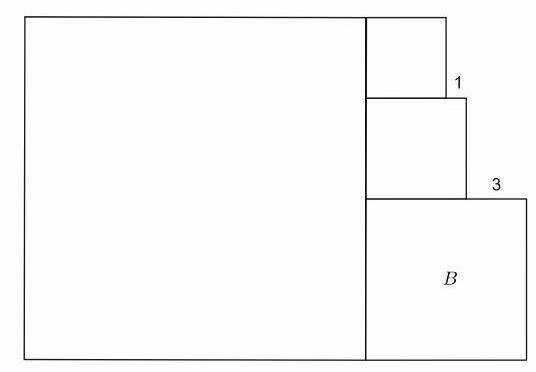
\includegraphics[max width=\textwidth, center]{2024_11_21_9c11f7163a8aec513b60g-1}

\section*{ZADANIE 3.}
W skarbonce Adama są tylko monety pięćdziesięciogroszowe i dziesięciogroszowe. Wszystkich monet jest 40. Pewnego dnia chłopiec rozmienił połowę posiadanych pięćdziesięciogroszówek na dziesięciogroszówki i teraz ma w skarbonce 60 monet. Ile dziesięciogroszówek jest wśród nich?

\section*{ZADANIE 4.}
W niektóre pola tablicy wpisano 0 . W pozostałe puste pola wpisz dwie jedynki, dwie dwójki, dwie trójki i dwie czwórki tak, aby suma liczb w każdym wierszu i w każdej kolumnie była taka sama. Czy jest tylko jeden sposób uzupełnienia tablicy? Odpowiedź uzasadnij.

\begin{center}
\begin{tabular}{|l|l|l|l|}
\hline
 & 0 & 0 &  \\
\hline
0 &  &  & 0 \\
\hline
 & 0 & 0 &  \\
\hline
0 &  &  & 0 \\
\hline
\end{tabular}
\end{center}

\section*{ZADANIE 5.}
Ile cyfr ma najdłuższy możliwy ciąg cyfr nie zawierający cyfry 0 , w którym każde dwie kolejne cyfry tworzą liczbę będącą kwadratem liczby naturalnej?


\end{document}